% !TeX spellcheck = en_GB
\documentclass[11pt,fleqn]{article}

\usepackage[english]{babel}
\usepackage{SpeedyGonzales}
\usepackage{MediocreMike}
%\usepackage{Blastoise}
\usepackage{listings}

\usepackage{float}
\usepackage[caption = false]{subfig}
\title{}
\author{Asger Schultz}
\date{\today}

\fancypagestyle{plain}
{
	\fancyhf{}
	\rfoot{Side \thepage{} af \pageref{LastPage}}
	\renewcommand{\headrulewidth}{0pt}
}
\pagestyle{fancy}
\fancyhf{}
\lhead{Asger Schultz}
\chead{}
\rhead{}
\rfoot{Side \thepage{} af \pageref{LastPage}}

\graphicspath{{Billeder/}}
\linespread{1.15}


%\numberwithin{equation}{section}
%\numberwithin{footnote}{section}
%\numberwithin{figure}{section}
%\numberwithin{table}{section}

\begin{document}

\maketitle
%\thispagestyle{fancy}
%\tableofcontents
\tableofcontents
\newpage 


\section{Introduction}
The field of artificial intelligence and machine learning is known for recognising patterns in high-dimensional data. 
One application of such modelling is in human identification as facial recognition and biometric scanning are becoming a large part of our every day for better and for worse. One, more subtle identifier is our bodily movement which can be imagined to vary between people.

It is thus an obvious question whether the difference in movement between people is enough to identify them. Achieving accurate modelling and a good understanding of such motor data might help fields such kinesiology and biomechanics and be applied in health and sport \cite{kine}.

Two simple machine learning models, a classification tree and a 3-nearest neighbour classifier, are tested on this human classification task in a single arm movement experiment where subects moved cylinders of different sizes and weights over obstacles. Furthermore, a statistical test is performed on 16 arm movement experiments to test whether the type of task was signficantly different.

\section{Data}
The data consists of 16 experiments where ten right-handed people had to move a cylinder over another cylinder.
The size and weight of the cylinders varied over the experiments, and each person had to perform the movement of each experiment 10 times.
Thus, the data was structured in a $ 16\times 10\times 10 $ array, with axes: experiment\(\times\)person\(\times\)repetition.
For every such repetition, the $ x, y, $ and $ z $ coordinates of the movement where recorded 100 times, such that the data for each repetition was a $ 100\times 3 $ matrix.
The data had been preprocessed such that every curve was of the same length.
Some of the movements are plotted in figure \ref{fig:trajects}.
\begin{figure}[H]
	\centering
	\subfloat{
		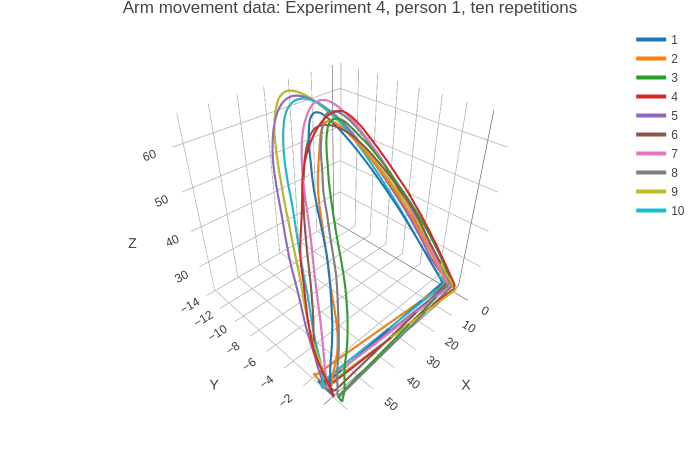
\includegraphics[width=.5\linewidth]{p1_3d_example1}
	}
	\subfloat{
		\centering
		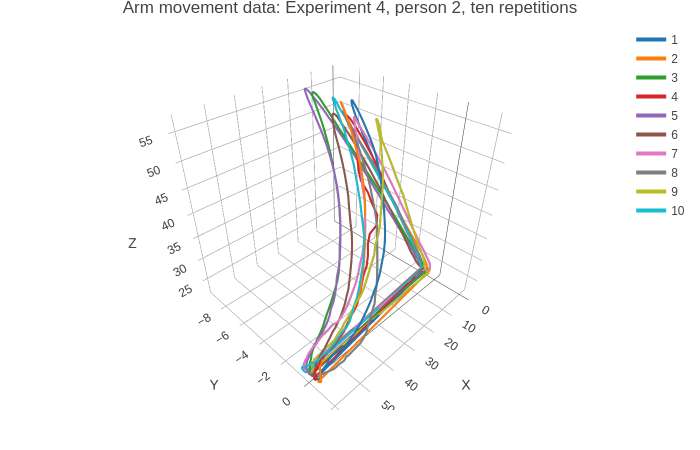
\includegraphics[width=.5\linewidth]{p1_3d_example2}
	}
	\label{fig:trajects}
	\caption{Hand movements of two different people in the fourth experiment.}
\end{figure}

\noindent 
For our purposes, it was benificial to consider each recording of $ x, y, $ and $ z $ a set of three features, so we ravelled the data such that each repetition had $ 300 $ features with one observation each.
For the first part of the report, we investigated only experiment 4, so we had a total of 100 observations.
The target variable was the person who performed the movement, so the goal of our machine learning models was a 10-class classification.

Later, we tested wether or not the experiment had a significant effect.
For this, we ravelled the data points into a vector of length $ 480,000 $, which is explained in more details in section \ref{subsec:expeffect}.


\section{Methods and analysis}


\subsection{Machine Learning Task: Classification}
Two machine learning models were chosen to test on this 300-dimensional 10-class data.
It is noted from initial plots -- fig. \ref{fig:trajects} and fig. \ref{fig:2dtrajects} -- that the effects of different people seem non-linear, such that models that can model nonlinear decision boundaries are considered.
\paragraph{Models} The two chosen models were a binary classification tree and a 3-nearest neighbour classifier. The classification tree used the implementation of Hunt's algorithm of the \texttt{tree} package in \texttt{R} \cite{Tree}. For splitting criterion, the \textit{deviance} is used which is based on minus two times the log likelihood of the data under each model that the split results in \cite{Deviance}.

The second model was the \(K\)-nearest neighbour classifier which predicts classes using \(K\) nearest data points in the training set in euclidean distance and tie breaking by increasing \(K\) for the data point as implemented in the \texttt{R} package \texttt{class} \cite{KNN}. Before training on the data set, the hyper parameters of both models were defined and were not subject for testing. \(K\) set to 3 as it was deemed suitable for the 10-class setting.

To evaluate the performance of the models, a classification baseline was set. As the classes are perfectly balanced, a baseline is expected to reach 10\pro\ accuracy. As no class is the largest, the baseline is constructed by randomly guessing classes to avoid skewing the evaluation towards any class as this might make a difference for the McNemar test.
\paragraph{Performance evaluation}
To evaluate which machine learning model best predicts which person completed the tasks, leave-one-out cross validation is implemented thus training the models on 99 data points and and testing on the last for each fold.
From here, 100 predictions are obtained which are used to achieve a point estimate for the accuracy of the classifiers.

To test whether the differences in the accuracy estimates are significant, McNemar's test is used. 
This test is used as described in \cite[Method 11.3.2]{Tue} and uses the beta distribution as a posterior to achieve a method for computing confidence interval of the difference in classifier accuracy.
From this test, a \(p\)-value for the null hypothesis that the two classifiers have the same accuracy can also be computed by using the binomial cumulative probability density function.

These tests consider the matched-pair matrix which counts the number of times the classifiers both are wrong, the number of times they both are right, the number of times one is better than the other (\(n_{12}\)) and vice versa (\(n_{21}\)).
Intuitively, this takes into account that some classifications might be more difficult than others. 
This is the motivation for the random baseline. It is noted that these parametric comparisons are approximations and \cite{Tue} states that the \(p\)-values and confidence intervals should be considered together and that they only hold when \(n_{12}+n_{21}> 5\).
\subsection{Test of experiment effect}\label{subsec:expeffect}
Analysis of Variance, or ANOVA, is a method for comparing the means of multiple groups.
This makes it useful for detecting if there is a significant difference between the experiments.
ANOVA works by testing the likelihood of a given mean's distance to the overall mean is due to random variation, which is done using variability decomposition.
We assumed the null hypothesis $ H_0: \mu_1=\mu_2=\ldots=\mu_{16} $.

In order to use ANOVA, all the 480,000 data points were ravelled into a vector of the same length.
Four similar vectors where then created for the explanatory variables.
The first contained the coordinates features, such as \texttt{z3} for the third $ z $-value.
The second contained the person, the third the repetition, and the fourth the experiment number.
We then used a linear model with R's \texttt{lm} function followed by \texttt{anova} to perform a four-way ANOVA (given the four explanatory factors).

One major assumption of ANOVA is that the residuals are normally distributed.
As figure \ref{fig:qq} shows, this is somewhat true, but with many exceptions, so the results should be taken with a grain of salt.
\begin{figure}[H]
	\centering
	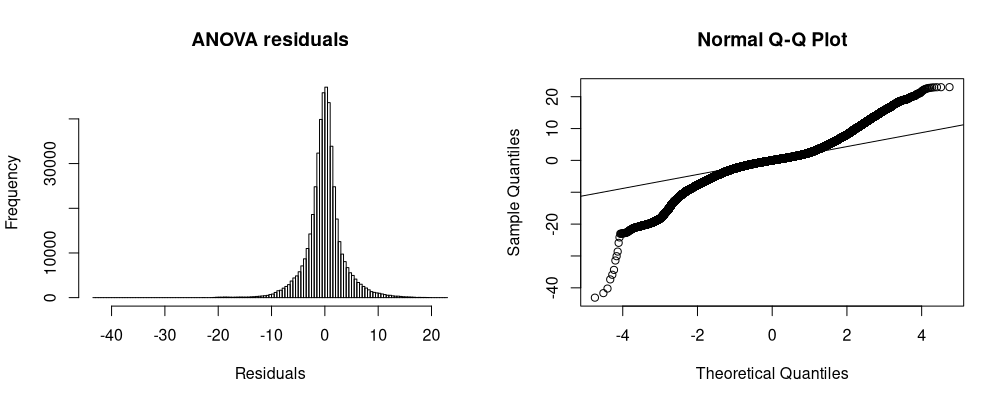
\includegraphics[width=.5\textwidth]{qq}
	\caption{Histogram and QQ-plot of the residuals of a linear model.}\label{fig:qq}
\end{figure}

\section{Results}

\subsection{Classification models}

\paragraph{Point estimates for accuracy}

\begin{align*}
	& \hat \theta_{Base}= 12\pro 
	&& \hat \theta_{Tree} =41\pro 
	&&&\hat \theta_{3NN} = 60 \pro 
\end{align*}
\paragraph{Comparison of 3NN and classification tree}
Matched pair matrix:

\begin{table}[H]
	\centering
	\begin{tabular}{l|c c}
		&Tree is correct& Tree is wrong \\
		\hline
		3NN is correct &35& 25\\
		3NN is wrong& 6& 34
	\end{tabular}
\end{table}\noindent 
Estimate for accuracy difference, 99\pro\ confidence interval and \(p\)-value for \(H_0: \theta_{3NN}=\theta_{Tree}\):
\[
\widehat{\Delta \theta} = 19\pro,\quad  \Delta \theta\in[7\pro , 30\pro], \quad p = 0.0059 
\]

\paragraph{Comparison of 3NN and baseline}
Matched pair matrix:

\begin{table}[H]
	\centering
	\begin{tabular}{l|c c}
		&Baseline is correct& Baseline is wrong \\
		\hline
		3NN is correct &7& 53\\
		3NN is wrong& 5& 35
	\end{tabular}
\end{table}\noindent 
Estimate for accuracy difference, 99\pro\ confidence interval and \(p\)-value for \(H_0: \theta_{3NN}=\theta_{Base.}\):
\[
\widehat{\Delta \theta} = 48\pro,\quad  \Delta \theta\in[33\pro , 61\pro], \quad p = 3.5\ctp{-11}
\]
\paragraph{Comparison of classification tree and baseline}
Matched pair matrix:

\begin{table}[H]
	\centering
	\begin{tabular}{l|c c}
		&Baseline is correct& Baseline is wrong \\
		\hline
		Tree is correct &2& 39\\
		Tree is wrong& 10& 49
	\end{tabular}
\end{table}\noindent 
Estimate for accuracy difference, 99\pro\ confidence interval and \(p\)-value for \(H_0: \theta_{Tree}=\theta_{Base.}\):
\[
\widehat{\Delta \theta} = 29\pro,\quad  \Delta \theta\in[14\pro , 43\pro], \quad p = 3.8\ctp{-5}
\]

\paragraph{Impact of experiment}
All experiments are seen to be significant at a significance level of $ \alpha=0.1\pro $.
\begin{table}[H]
	\centering
	\begin{tabular}{lrrrrr}
		          &     Df&    Sum Sq& Mean Sq&   $ F $ value&    Pr($ < $F)    \\
		coordinate&    299& 230298000&  770227& 61477.804&  $ < $2.2e-16 ***\\
		repetition&      9&     10036&    1115&    89.007&  $ < $2.2e-16 ***\\
		person    &      9&    124551&   13839&  1104.595&  $ < $2.2e-16 ***\\
		experiment&     15&    433652&   28910&  2307.543&  $ < $2.2e-16 ***\\
		Residuals & 479631&   6009079&      13& &
	\end{tabular}
	\caption{R output from ANOVA. Three asterisks mean significance at a significance level of $ \alpha=0.1\pro $.}\label{tab:ranova}
\end{table}
\begin{table}[H]
	\centering
	\begin{tabular}{lrrrr}
		&Estimate &Std. Error &$ t $ value &Pr($ >|t| $)\\
		(Intercept)&    -1.158886&   0.093391& -12.409&  $ < $ 2e-16 ***\\
		experiment2&     0.361933&   0.028900&  12.523&  $ < $ 2e-16 ***\\
		experiment3&     1.122695&   0.028900&  38.847&  $ < $ 2e-16 ***\\
		experiment4&     0.252041&   0.028900&   8.721&  $ < $ 2e-16 ***\\
		experiment5&     0.710498&   0.028901&  24.584&  $ < $ 2e-16 ***\\
		experiment6&     1.442134&   0.028900&  49.900&  $ < $ 2e-16 ***\\
		experiment7&     0.488445&   0.028901&  16.901&  $ < $ 2e-16 ***\\
		experiment8&     1.161682&   0.028900&  40.196&  $ < $ 2e-16 ***\\
		experiment9&     1.843712&   0.028900&  63.795&  $ < $ 2e-16 ***\\
		experiment10&    0.703864&   0.028902&  24.354&  $ < $ 2e-16 ***\\
		experiment11&    1.592115&   0.028902&  55.087&  $ < $ 2e-16 ***\\
		experiment12&    2.500064&   0.028900&  39.275&  $ < $ 2e-16 ***\\
		experiment14&    2.103468&   0.028902&  72.780&  $ < $ 2e-16 ***\\
		experiment15&    3.219295&   0.028900& 111.393&  $ < $ 2e-16 ***\\
		experiment16&   -0.612838&   0.028900& -21.205&  $ < $ 2e-16 ***
	\end{tabular}
	\caption{R output from the summary of the linear model concerning the impacts of the experiments.}
\end{table}\noindent

\section{Discussion and Conclusion}
\subsection{Classification of persons}
%The initial visualizations of the data in the 3D and 2D scatter plots -- \ref{fig:trajects} and \ref{fig:2dtrajects} -- showed clear differences between the repetitions of the first two people that humans would be able to classify visually especially it is seen that there is a clear difference in the way these two people move in the \(y\)-direction.  
It is seen that the expectation of some accuracy was confirmed: The 3-nearest neighbour model is the best at 60\pro\ and is significantly better than the classification tree and they are both significantly better than the random guesses. The greater aim of reliably discerning people based on movement is far from achieved at an performance of 60\pro. However, this significant result with these un-optimized models shows a promise for the machine learning task as there is a number of possible improvements. 



The models were not tested for complexity controlling hyper parameters such as \(K\) for the KNN or the impurity function for the tree model and possible improvements could be found here. A larger improvement could be found in much more complex models for this high-dimensional data set such as random forests or deep neural networks. More generalizable performance could also be found by using the entire data set, not just experiment 4, to find more general personal  features and mannerisms.

\subsection{Test of difference in experiments}
We found that the experiment had a statistically significant impact on the hand movements of the test subjects with $ p<2.2\ctp{-16} $.
This was also the case for every individual experiment.
However, the assumptions of the ANOVA test utilized were not fully realized (see figure \ref{fig:qq}), which is likely to have had at least some impact on the test.
Combined with the 480,000 data points, this could help explain the exceptionally low $ p $ values.
The unfulfilled assumptions could also help explain one of the more surprising results of the experiments: That the repetition also had a $ p $ value of less than $ 2.2\ctp{-16} $.
As seen on table \ref{tab:ranova}, most of the variance was explained by the coordinate variable, which is not surprising.

\begin{thebibliography}{9}
	\bibitem{Tue} Herlau, Tue et al. "Introduction to Machine Learning and Data Mining: Lecture notes, Fall 2019, version 1.4b" 13/12-19.
		\bibitem{kine} The University of British Columbia: School of Kinesiology:
	"Neuromechanical Studies in Kinesiology". \\
	At:
	\url{https://kin.educ.ubc.ca/research/neuro-mechanical/} (consulted 19/01-20)
	\bibitem{KNN} Ripley, Brian: "Package ’class’", 01/01-19 .\\
	At:
	
	\url{https://cran.r-project.org/web/packages/class/class.pdf} (consulted 16/01-20)
	\bibitem{Tree} Ripley, Brian: "Package ‘tree’", 26/05-19.\\ At: \url{https://cran.r-project.org/web/packages/tree/tree.pdf} (consulted 16/01-20)
	\bibitem{Deviance} Ritschard, Gilbard: "Computing and using the deviance with classification trees", 01-06.\\
	 At:
	\url{http://mephisto.unige.ch/pub/publications/gr/ritschard_compstat06.pdf} (consulted 16/01-20)

\end{thebibliography}
\appendix
\section{Figures}
\begin{figure}[H]
	
	\centering
	\subfloat{
		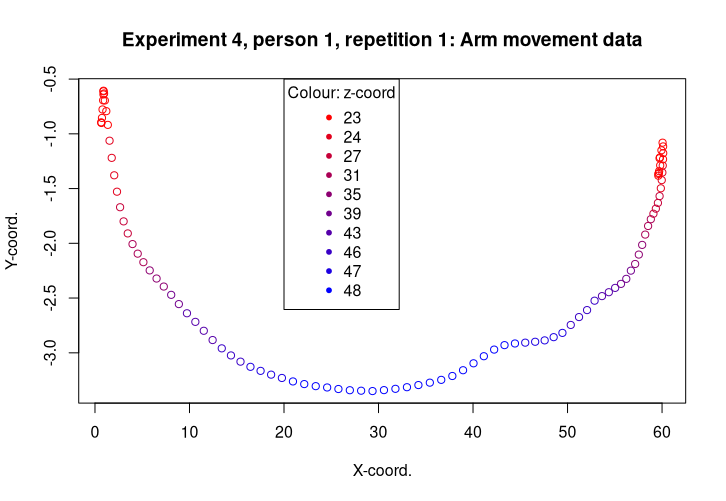
\includegraphics[width=.5\linewidth]{p1_example}
	}
	\subfloat{5
		\centering
		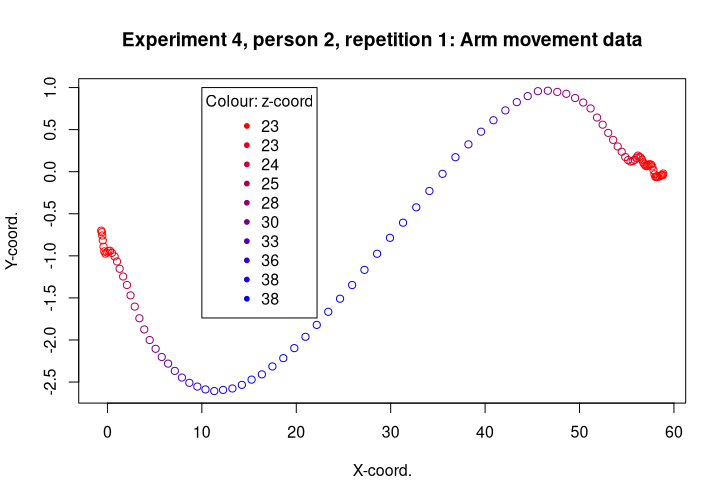
\includegraphics[width=.5\linewidth]{p1_example2}
	}
	\caption{Floats}
	\label{fig:2dtrajects}
\end{figure}


\end{document}

















